\documentclass{standalone}
\usepackage{tikz}
\begin{document}
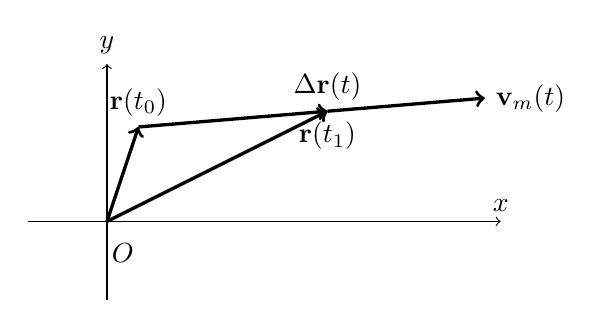
\begin{tikzpicture}[scale = 2]
    \coordinate (O) at (0,0);
    \node[black] at (0.1, -0.2) {$O$};
    \draw[->] (-0.5, 0) -- (2.5, 0) coordinate (x) node[above]{$x$};
    \draw[->] (0,-0.5) --(0,1) coordinate (y) node[above]{$y$};
    \draw[->,very thick] (O) -- (0.2, 0.6) node[above] {$\mathbf{r}(t_0)$};
    \draw[->,very thick] (O) -- (1.4, 0.7) node[below] {$\mathbf{r}(t_1)$};
    \draw[->,very thick] (0.2, 0.6) -- (1.4, 0.7) node[above] {$\Delta\mathbf{r}(t)$};
    \draw[->,very thick] (1.4, 0.7) -- (2.4,47/60) node[right] {$\mathbf{v}_m(t)$};
\end{tikzpicture}
\end{document}